% Created 2022-05-25 Wed 23:40
% Intended LaTeX compiler: pdflatex
\documentclass[t,10pt,xcolor={dvipsnames}]{beamer}
\usepackage[utf8]{inputenc}
\usepackage[T1]{fontenc}
\usepackage{graphicx}
\usepackage{grffile}
\usepackage{longtable}
\usepackage{wrapfig}
\usepackage{rotating}
\usepackage[normalem]{ulem}
\usepackage{amsmath}
\usepackage{textcomp}
\usepackage{amssymb}
\usepackage{capt-of}
\usepackage{hyperref}
\definecolor{Orange}{rgb}{1,0.5,0}
\usepackage{listings}
%%%% listings pkg: %%%%

% \lstloadlanguages{Haskell}

\lstset{
  basicstyle=\scriptsize\ttfamily,
  %mathescape=true,
  %numbers=left,
  mathescape=false,
  aboveskip=\medskipamount,
  belowskip=\smallskipamount,
  showspaces=false,
  keywordstyle=,
  numberstyle=\tiny,
  numbersep=0pt,
  %stepnumber=2,
  tabsize=2,
  %extendedchars=true,
  breaklines=false,
  %keywordstyle=\color{black}
  }
  % TODO this inherited or not from other lstnewenvironment
\newcommand{\lstcd}[1]{\lstinline[basicstyle=\ttfamily\footnotesize]{#1}}

% this style is used for long/verbatim notes (not text) in the paper
\lstdefinestyle{meta}
  {basicstyle=\scriptsize\ttfamily\color{magenta}}

\lstnewenvironment{myc}
    {\lstset{}%
      \csname lst@SetFirstLabel\endcsname}
    {\csname lst@SaveFirstLabel\endcsname}
    \lstset{
      basicstyle=\scriptsize\ttfamily,
      mathescape=false,
      language=C,
      lineskip=1pt,
      showspaces=false,
      keywordstyle=,
      flexiblecolumns=false,
      basewidth={0.5em,0.45em}
    }

\lstnewenvironment{code}
    {\lstset{}%
      \csname lst@SetFirstLabel\endcsname}
    {\csname lst@SaveFirstLabel\endcsname}
    \lstset{
      mathescape=false,
      language=Haskell,
      lineskip=1pt,
      showspaces=false,
      numbersep=0pt,
      keywordstyle=,
      basicstyle=\scriptsize\ttfamily,
      flexiblecolumns=false,
      basewidth={0.5em,0.45em},
      literate={+}{{$+$}}1 {/}{{$/$}}1 {*}{{$*$}}1 {=}{{$=$}}1
               {>}{{$>$}}1 {<}{{$<$}}1 {\\}{{$\lambda$}}1
               {\\\\}{{\char`\\\char`\\}}1
               {->}{{$\rightarrow$}}2 {>=}{{$\geq$}}2 {<-}{{$\leftarrow$}}2
               {<=}{{$\leq$}}2 {=>}{{$\Rightarrow$}}2 
          %     {\ .\ }{{$\circ$}}2
               {>>}{{>>}}2 {>>=}{{>>=}}2
               {|}{{$\mid$}}1               
    }
    % literate haskell assumes \begin{code}

% when we don't want Haskell to execute the code in paper:
% Alts    
%   \newenvironment{codeNoExecute}{\code}{\endcode} 
%   \let\codeNoExecute\code
%   \let\endcodeNoExecute\endcode
%   the below, just duplicated from above:
\lstnewenvironment{codeNoExecute}
    {\lstset{}%
      \csname lst@SetFirstLabel\endcsname}
    {\csname lst@SaveFirstLabel\endcsname}
    \lstset{
      mathescape=false,
      language=Haskell,
      lineskip=1pt,
      showspaces=false,
      keywordstyle=,
      basicstyle=\scriptsize\ttfamily,
      flexiblecolumns=false,
      basewidth={0.5em,0.45em},
      literate={+}{{$+$}}1 {/}{{$/$}}1 {*}{{$*$}}1 {=}{{$=$}}1
               {>}{{$>$}}1 {<}{{$<$}}1 {\\}{{$\lambda$}}1
               {\\\\}{{\char`\\\char`\\}}1
               {->}{{$\rightarrow$}}2 {>=}{{$\geq$}}2 {<-}{{$\leftarrow$}}2
               {<=}{{$\leq$}}2 {=>}{{$\Rightarrow$}}2 
           %   {\ .\ }{{$\circ$}}2
               {>>}{{>>}}2 {>>=}{{>>=}}2
               {|}{{$\mid$}}1               
    }
    % literate haskell assumes \begin{code}

    
\usepackage{hyperref}
\usepackage[capitalise]{cleveref}
  % i.e., you use '\cref{x}' rather than "Figure \ref{x}"
% inlined bib file
\usepackage{filecontents}

% SYSTEM OF ANNOTATIONS:

\newcommand{\pwnote}[1]{\textcolor{blue}{[PW: #1]}}
\newcommand{\mtnote}[1]{\textcolor{BlueGreen}{[MT: #1]}}
\newcommand{\whnote}[1]{\textcolor{Cyan}{[WH: #1]}}
\newcommand{\wwnote}[1]{\textcolor{orange}{[WW: #1]}}

\newcommand{\pwtodo}[1]{\pwnote{TODO: #1}}
\newcommand{\mttodo}[1]{\mtnote{TODO: #1}}
\newcommand{\whtodo}[1]{\whnote{TODO: #1}}


\newcommand{\info}[1]{\textcolor{brown}{[[#1]]}}
\newcommand{\note}[1]{\noteYes{#1}}  
\newcommand{\noteNo}[1]{}  % way to remove all notes.
\newcommand{\noteYes}[1]{\textcolor{red}{[[#1]]}}
\newcommand{\todo}[1]{\note{TODO: #1}}
\newcommand{\todoa}[1]{\todo{[\#A]: #1}}
\newcommand{\todob}[1]{\todo{[\#B]: #1}}
\newcommand{\todoc}[1]{\todo{[\#C]: #1}}
\newcommand{\old}[1]{\textcolor{orange}{[[OLD: #1]]}}

\newcommand{\haskellnote}[1]{#1}
  % ever add formatting to? Just used to indicate notes to non-Haskellers
\newcommand{\keypoint}[1]{{\bf{#1}}}
  % TODO: boxed frame maybe?
\newcommand{\paragraphsection}[1]{\vspace{7pt}\noindent{\textit{#1}}}
  % use this for "Initial Results" or for sections at the lowest level.
  % TODO: is the formatting sufficiently smaller than level 2 sections?
 
\sisetup{group-separator={,}, group-minimum-digits=4}


\author{Mark Tullsen, William Harris, Peter Wyatt \\ \\ {tullsen,wrharris}@galois.com \\ peter.wyatt@pdfa.org }
\usetheme{Madrid}
\author{Mark Tullsen, William Harris, Peter Wyatt}
\date{May 26, 2022}
\title{Strengthening Weak Links in the PDF Trust Chain}
\hypersetup{
 pdfauthor={Mark Tullsen, William Harris, Peter Wyatt},
 pdftitle={Strengthening Weak Links in the PDF Trust Chain},
 pdfkeywords={},
 pdfsubject={},
 pdfcreator={Emacs 27.2 (Org mode 9.4.4)}, 
 pdflang={English}}
\begin{document}

\maketitle
\begin{frame}{Outline}
\tableofcontents
\end{frame}

\section{Pre-DOM (Pre Document Object Model)}
\label{sec:orged562a7}
\begin{frame}[label={sec:org7a09591}]{PDF Complexity?}
\begin{center}
 { \hspace{5pt}
   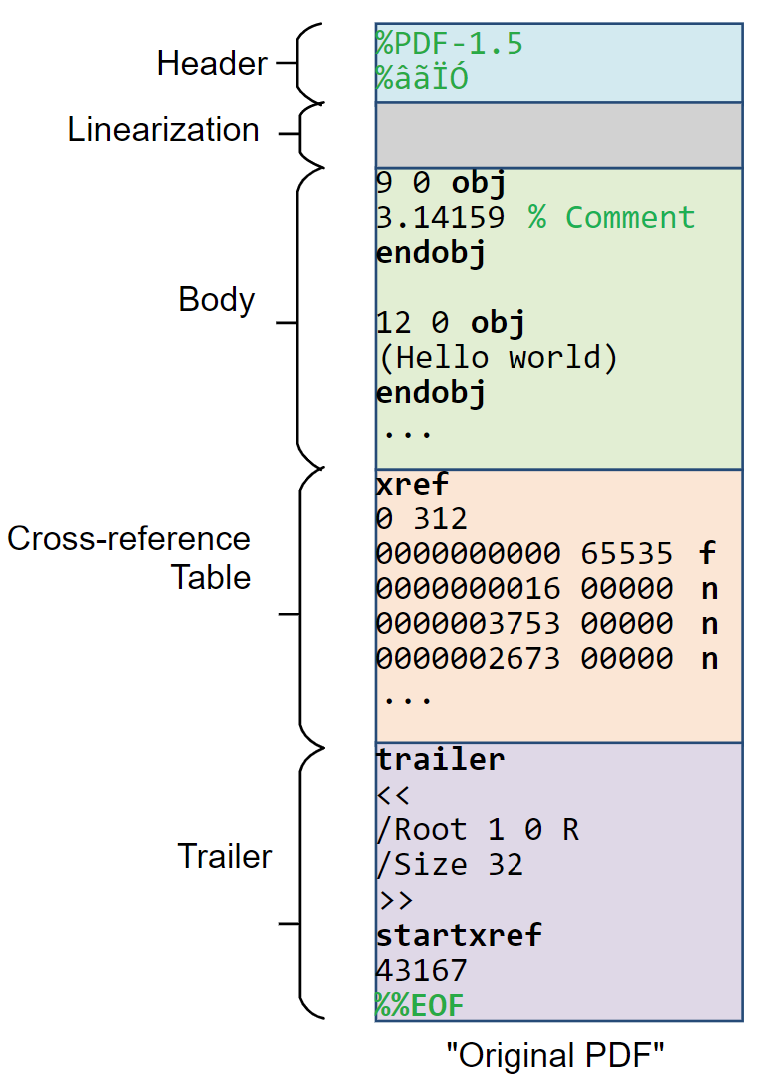
\includegraphics[width=0.4\linewidth]{../figures/pdf-structure.png}
 } \hspace{30pt}
 \raisebox{-1\baselineskip}
          {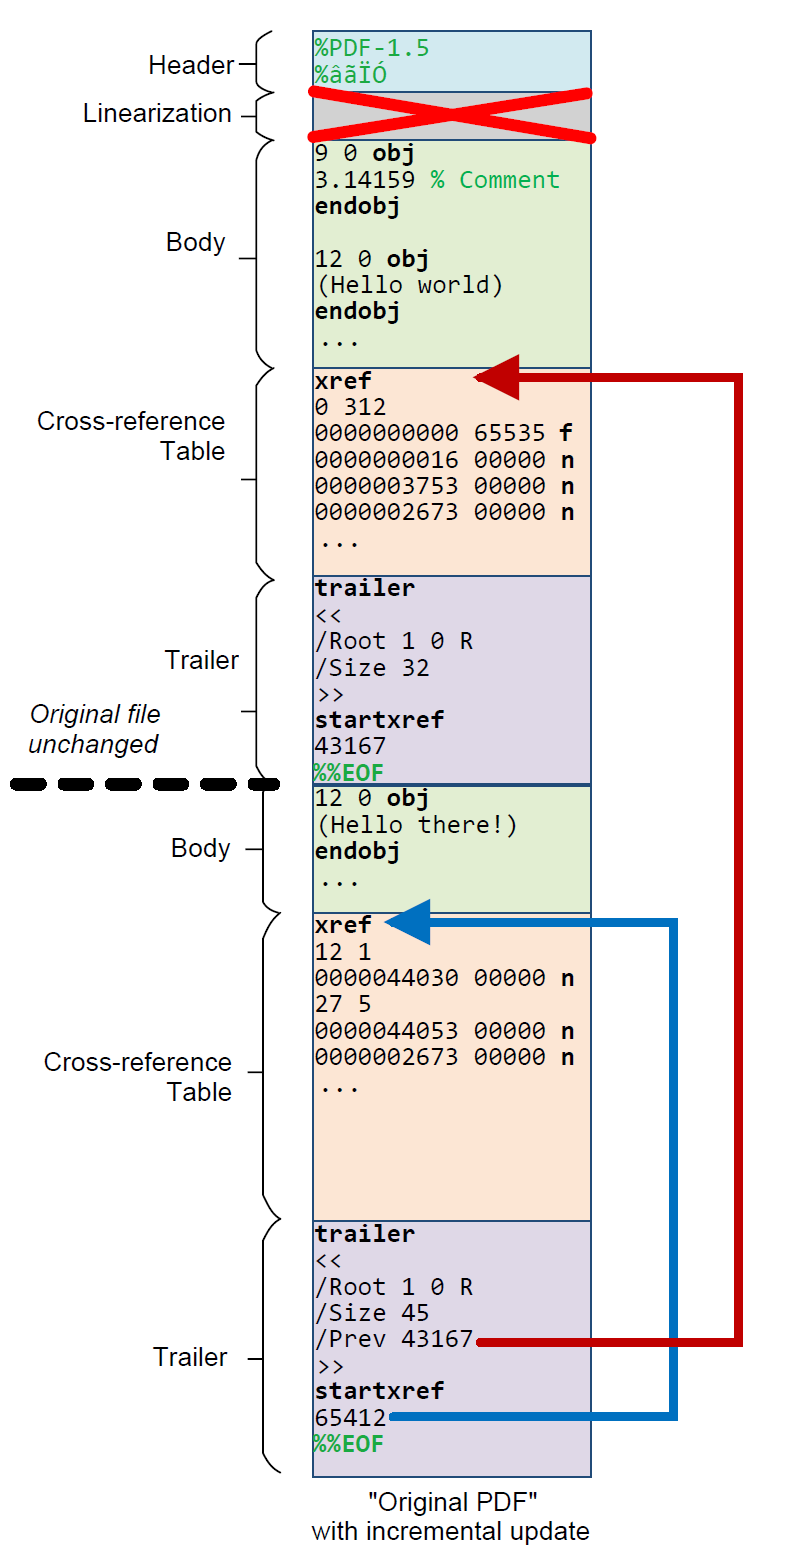
\includegraphics[width=0.30\linewidth]{../figures/pdf-structure-incremental.png}}
\end{center}
\end{frame}

\begin{frame}[label={sec:org48cfdec}]{PDF Trust Chain: Pre-DOM and Post-DOM}
\begin{center}
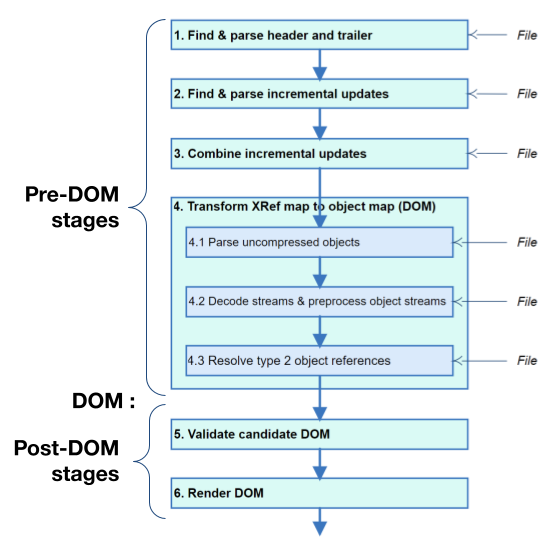
\includegraphics[width=0.63\linewidth]{images/trustchain-with-braces.png}
\end{center}
\end{frame}

\begin{frame}[label={sec:org82d4664}]{Vulnerabilities Occurring Primarily Pre-DOM}
\begin{itemize}
\item Schizophrenic files (different tools, different renderings)
\item Polyglot files (file being in 2+ formats)
\item Shadow attacks
\begin{itemize}
\item i.e., attacker can
\begin{itemize}
\item add "shadow content" that is PDF-signed,
\item after signing, can update-at-will (revealing shadow content)
\item without giving clear warnings to user.
\end{itemize}
\item possible because of ability to sign \emph{dead objects} and \emph{cavities}
\end{itemize}
\item Multiple places for hidden/unused/malicious data in PDF
\begin{itemize}
\item non-obvious places, unnoticed when "simply parsing"
\item e.g., shadow-attacks
\item dead bytes, dead objects, dead updates, dead linearization sections, etc.
\end{itemize}
\end{itemize}
\end{frame}

\section{Modeling Pre-DOM: Highlights}
\label{sec:org9a1651f}
\begin{frame}[label={sec:org9913ba2},fragile]{Stage 4 Sub-Stages: Transform XRef Map to Object Map}
\vspace*{-15pt}
\begin{center}
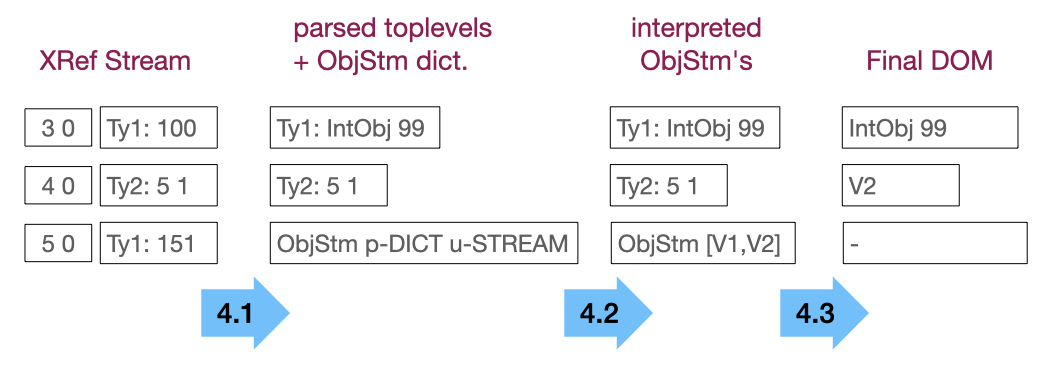
\includegraphics[width=0.75\linewidth]{images/diagram1/cropped-diagram1.001.png}
\end{center}
\vspace*{-15pt}
\begin{lstlisting}[style=pdfcode]
        ... 
  100   3 0 obj 99 endobj
  123   % object 4 is not here
  151   5 0 obj
        <<
        /Type /ObjStm
        /Length 3 0 R   % indirect!
        /N 2            % 2 objects; (potentially indirect)
        /First 10       % offset to 1st object (potentially indirect)
        >>
        stream
        4 0 6 100
        V1 % PDF-Value here, 4 0 R, [fake comment] 
        V2 % PDF-Value here, 6 0 R, [fake comment]
        endstream
        endobj
  409   7 0 obj ... endobj
        ...
\end{lstlisting}
\end{frame}

\begin{frame}[label={sec:orga668446}]{Parser \(\neq\) Validator}
\begin{itemize}
\item A surprising source of mis-communication.
\item \ldots{}
\end{itemize}
\end{frame}
\begin{frame}[label={sec:orga72adad}]{A Validator (Parser \(\neq\) Validator)}
\vspace{10pt}
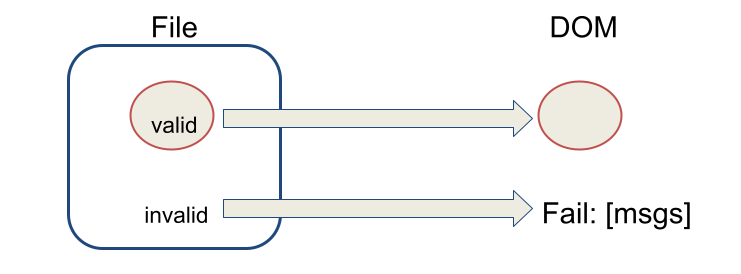
\includegraphics[width=0.80\linewidth]{images/pNEQv-1.png}
\vfill

VALIDATOR: only valid PDFs can produce DOM (must Fail otherwise)
\end{frame}

\begin{frame}[label={sec:org9d6fb3c}]{A Parser (Parser \(\neq\) Validator)}
\vspace{10pt}
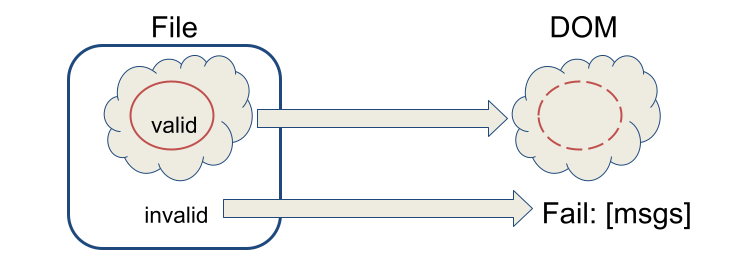
\includegraphics[width=0.80\linewidth]{images/pNEQv-2.png}
\vfill

PARSER: efficiently, construct the correct DOM when a valid PDF
\end{frame}

\begin{frame}[label={sec:org7d79748}]{A Very Accepting Parser (Parser \(\neq\) Validator)}
\vspace{10pt}
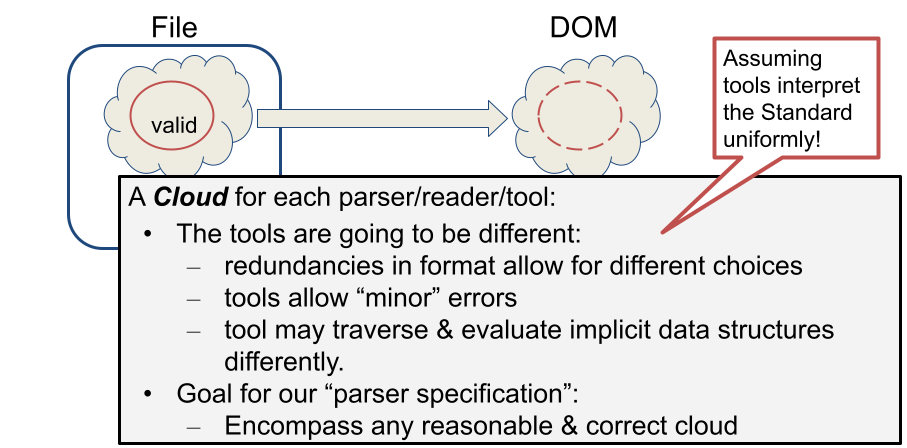
\includegraphics[width=0.95\linewidth]{images/pNEQv-3.png}
\end{frame}

\begin{frame}[label={sec:orgcfc1e0a},fragile]{Turning Parser into Validator}
 Parser specification is designed to be
\begin{itemize}
\item understandable: clear, pure Haskell
\item phased, clearly terminating (get parallelizability for free)
\item very lazy "Parser" (big input cloud)
\end{itemize}

We can extend spec into a validator, orthogonally, via “validate” constructs
(turning on/off on with command-line flag).  E.g.,
\lstset{language=haskell,label= ,caption= ,captionpos=b,numbers=none}
\begin{lstlisting}
do
(xrefRaw, xrefEndOff) <- pXrefRaw
validate $
   verifyXrefRaw xrefRaw -- ensures no duplicates
\end{lstlisting}
\end{frame}

\section{Conclusions}
\label{sec:org1dcc53c}
\begin{frame}[label={sec:orgebcb3d4}]{Accomplishments}
\begin{itemize}
\item A specification for pre-DOM parsing/computation
\begin{itemize}
\item Clarifies some subtle issues in PDF Standard
\item A growing list of PDF Association “issues” that we have contributed to
creating [23,24,\ldots{},30]
\end{itemize}
\item Cause \emph{and} effect of
\begin{itemize}
\item unique tool for displaying updates \& cavities
\end{itemize}
\end{itemize}
\end{frame}

\begin{frame}[label={sec:org788cc86}]{Future}
\begin{itemize}
\item Not accomplished yet
\begin{itemize}
\item the less interesting/subtle parts specified/implemented
\item integrated with our primitive, daedalus-generated parsers to create
a  tool.
\end{itemize}

\item Create a full pre-DOM tool that
\begin{itemize}
\item supports further PDF features (hybrids, compression, …)
\item add support for commonly allowed “exuberances”
\item add more “validate”s to get closer to a \emph{validator}.
\end{itemize}
\end{itemize}
\end{frame}

\section{Preview: Parser as API}
\label{sec:org3f054ca}
\begin{frame}[label={sec:orge3de404},fragile]{Implementation?}
 Tools \& renderers rarely need (\emph{demand}) the whole PDF
\begin{itemize}
\item reading?
\item parsing??
\item semantic checks???
\end{itemize}
\vspace{12pt}

Thus, this
\lstset{language=haskell,label= ,caption= ,captionpos=b,numbers=none}
\begin{lstlisting}
parsePDF :: FileData -> Maybe PDFAbstractSyntax
\end{lstlisting}
is not going to be used in practice!     
\end{frame}

\begin{frame}[label={sec:orgd9e8c39},fragile]{One Solution \ldots{}}
 \begin{itemize}
\item For complex formats,
\begin{itemize}
\item tools are "projections": rarely used parse/validate all.
\item may have alternate "parsing paths" we want to take
\begin{itemize}
\item e.g., metadata, page 1, text-only
\end{itemize}
\end{itemize}

\item Shotgun Parsers?
\begin{itemize}
\item \ldots{} the deadliest of patterns: "Input data checking, handling interspersed
with processing logic"
\end{itemize}

\item I.e., we provide multiple parsers where the following is interspersed through
code and the relation between these is \alert{not specified}:
\lstset{language=haskell,label= ,caption= ,captionpos=b,numbers=none}
\begin{lstlisting}
parseA :: Offset -> IO A
parseB :: Offset -> IO B
parseC :: Offset -> IO C
validateA :: A -> IO ()
validateB :: A -> B -> IO ()
\end{lstlisting}
\end{itemize}
\end{frame}

\begin{frame}[label={sec:orgaeb63a5},fragile]{Better Solution, Parser as API}
 We provide four inter-dependent calls (not \emph{entry points}):
\lstset{language=haskell,label= ,caption= ,captionpos=b,numbers=none}
\begin{lstlisting}
parseHdrTrlr :: FileData -> IO HdrTrlr
parseUpdates :: HdrTrlr -> IO [Updates]
createXRef   :: [Updates] -> IO XRef
derefObjId   :: ObjId -> XRef -> IO PdfValue
\end{lstlisting}
(The returned types can be as abstract as we wish.)

\vspace{18pt}

Using this, we write abstractions on the above:
\lstset{language=haskell,label= ,caption= ,captionpos=b,numbers=none}
\begin{lstlisting}
getInitialUpdate :: FileData -> IO XRef
getRootValue     :: HdrTrailer -> XRef -> PdfValue
getPageTree      :: XRef -> Tree PdfValue
\end{lstlisting}
\end{frame}
\end{document}
